\section{Methods} \label{sec:methods}%
\subsection{Physical problem of interest}
\label{subsec:physical_problem}
Consider a \ac{DUS} pulse as it travels into the lungs. The wave
traverses several layers of soft tissue and fluid that make up the
thoracic wall and pulmonary pleura. After passing through the pleurae,
the wave encounters a network of openly connected, air-filled saccules
with distinctly irregular surfaces. These are the alveoli. It is the
interaction between an incident \ac{US} pulse and the first alveolar
tissue-air interface it encounters, as illustrated in figure
\ref{fig:alveolar_schematic}\hl{MAKE A BETTER FIGURE}, to which we
focus our attention. For simplicity, we will model this problem using
acoustic wave traveling from soft tissue (treated as water) onto an
alveolus (treated as air). As we are motivated to study
\ac{DUS}-induced \ac{LH}, we will use the physical conditions relevant
to this problem to lend context to our study, though we will expand
the range of parameters we study to gain further insight study
acoustically driven interfaces.

There are several length and time scales relevant to this
problem. The reference length scale that we will use throughout the
rest of this work is the mean alveolar diameter $\ell$, which for
adult humans is about $\approx 200 \mu$m \citep{Ochs2004}. The
thoracic wall has mean anterior thickness ranging from $2.1$ - $2.3$
cm \cite{McLean2011}, such that the length of the fluid layer in front
of the alveolus $>>\ell$. The focal diameter of the ultrasound is at
minimum of the order of the ultrasonic wave $\lambda$, which is
$\approx 1$ mm for $1.5$ MHz \ac{US}, which has been found to cause
\ac{LH} in mice and rats \cite{Child1990,Miller2015a}. As this focal diameter is
appreciably larger than $\ell$, a flat alveolar interface will see the
incoming pulse as a spatially uniform plane wave. We will consider an
ultrasound pulse duration of approximately $5.5 \mu$s, which is
consistent with previous research \citep{Child1990}, and has a
corresponding spatial duration of $L=45\ell = 9$mm for a soft tissue sound
speed of $c=1649$ m/s. 

The lungs have long been recognized highly inhomogeneous, viscoelastic
organs \citep{Bayliss1939,Suki1994} with multiple physical effects at
play, including viscosity, elasticity, and surface tension. We perform
dimensional analyses to determine which of these are important over
the length and time scales relevant to the dynamics during
\ac{DUS}. In consideration of viscous effects, we calculate an
approximate length scale over which viscous effects will travel in the
tissue. To avoid the effects of multiple \ac{US} pulses, the longest
time span reasonable to observe the evolution of the system of is the
time between consecutive pulses, which for a typical pulse repetition
frequency of $1$ kHz is $t<\delta t_{pulse}=1000 \mu$ s. Due to
computational limitations, this work only considers the evolution of
the system up to $t\leq1000 \ell/c_{air}=576 \mu$s, such that the
viscous length will scale as
$L_{viscous}\sim\sqrt{\nu_{water} \delta t_{pulse}}=20 \mu$m. This is
appreciably less that $\ell$, and as we will demonstrate later,
appreciably less than some of the deformations we observe. Hence will
exclude the effects of viscosity in our calculations. In consideration
of surface tension in the lung, and which has been measured as $9$ mN/m
\citep{Schurch1976}, we define an acoustic Weber number for a
$p_a=1$ MPa acoustic wave amplitude such that
$We=p_a\ell/\sigma_{lung}=\orderof{10^4}>>1$, suggesting that the
acoustic forces during \ac{DUS} are far greater than those generated
by surface tension and as such we will neglect surface tension in our
model. Lastly, in consideration of the elasticity of the alveolar
wall, treated as $K = 5$ kPa \cite{Cavalcante2005}, we compute an
acoustic Cauchy number such that $Ca=p_a/K=200$, such that we neglect
the effects of elasticity in the lungs.
%
%
\subsection{Computational model}
\label{subsec:setup}
%
\begin{figure}[!h]
  \centering
  \begin{subfigure}[b]{0.45\textwidth}
    \centering
    \def\svgwidth{\textwidth}
    \import{./figs/lung_figs/}{Alveolus_US_zoom_only_diagram.pdf_tex} \hfill%
    \caption{\label{fig:alveolar_schematic} Physical problem of interest: an \ac{US} wave impinges upon an alveolus.}
  \end{subfigure}
  ~
  \begin{subfigure}[b]{0.45\textwidth}
    \centering
    \def\svgwidth{\textwidth}
    \import{./figs/lung_figs/}{usbe_model_schematic_domain.pdf_tex} \hfill%
    \caption{\label{fig:problem_schematics} A schematic of the model problem.}
  \end{subfigure}
  %
  \caption[A schematic view of the physical and model
  problems]{\protect\subref{fig:alveolar_schematic} illustrates the
    physical problem of interest, an ultrasound wave traveling into
    the lung and impinging upon the first alveolus it
    encounters. \protect\subref{fig:problem_schematic} shows the model
    problem, consisting of an acoustic wave impinging from water onto
    a sinusoidally interface with air.}
  \label{fig:schematics}
\end{figure}
% \begin{figure}[h]
%   \centering
%   \def\svgwidth{0.48\textwidth}
%    \import{./figs/lung_figs/}{Alveolus_US_zoom_only_diagram.pdf_tex} \hfill%
%    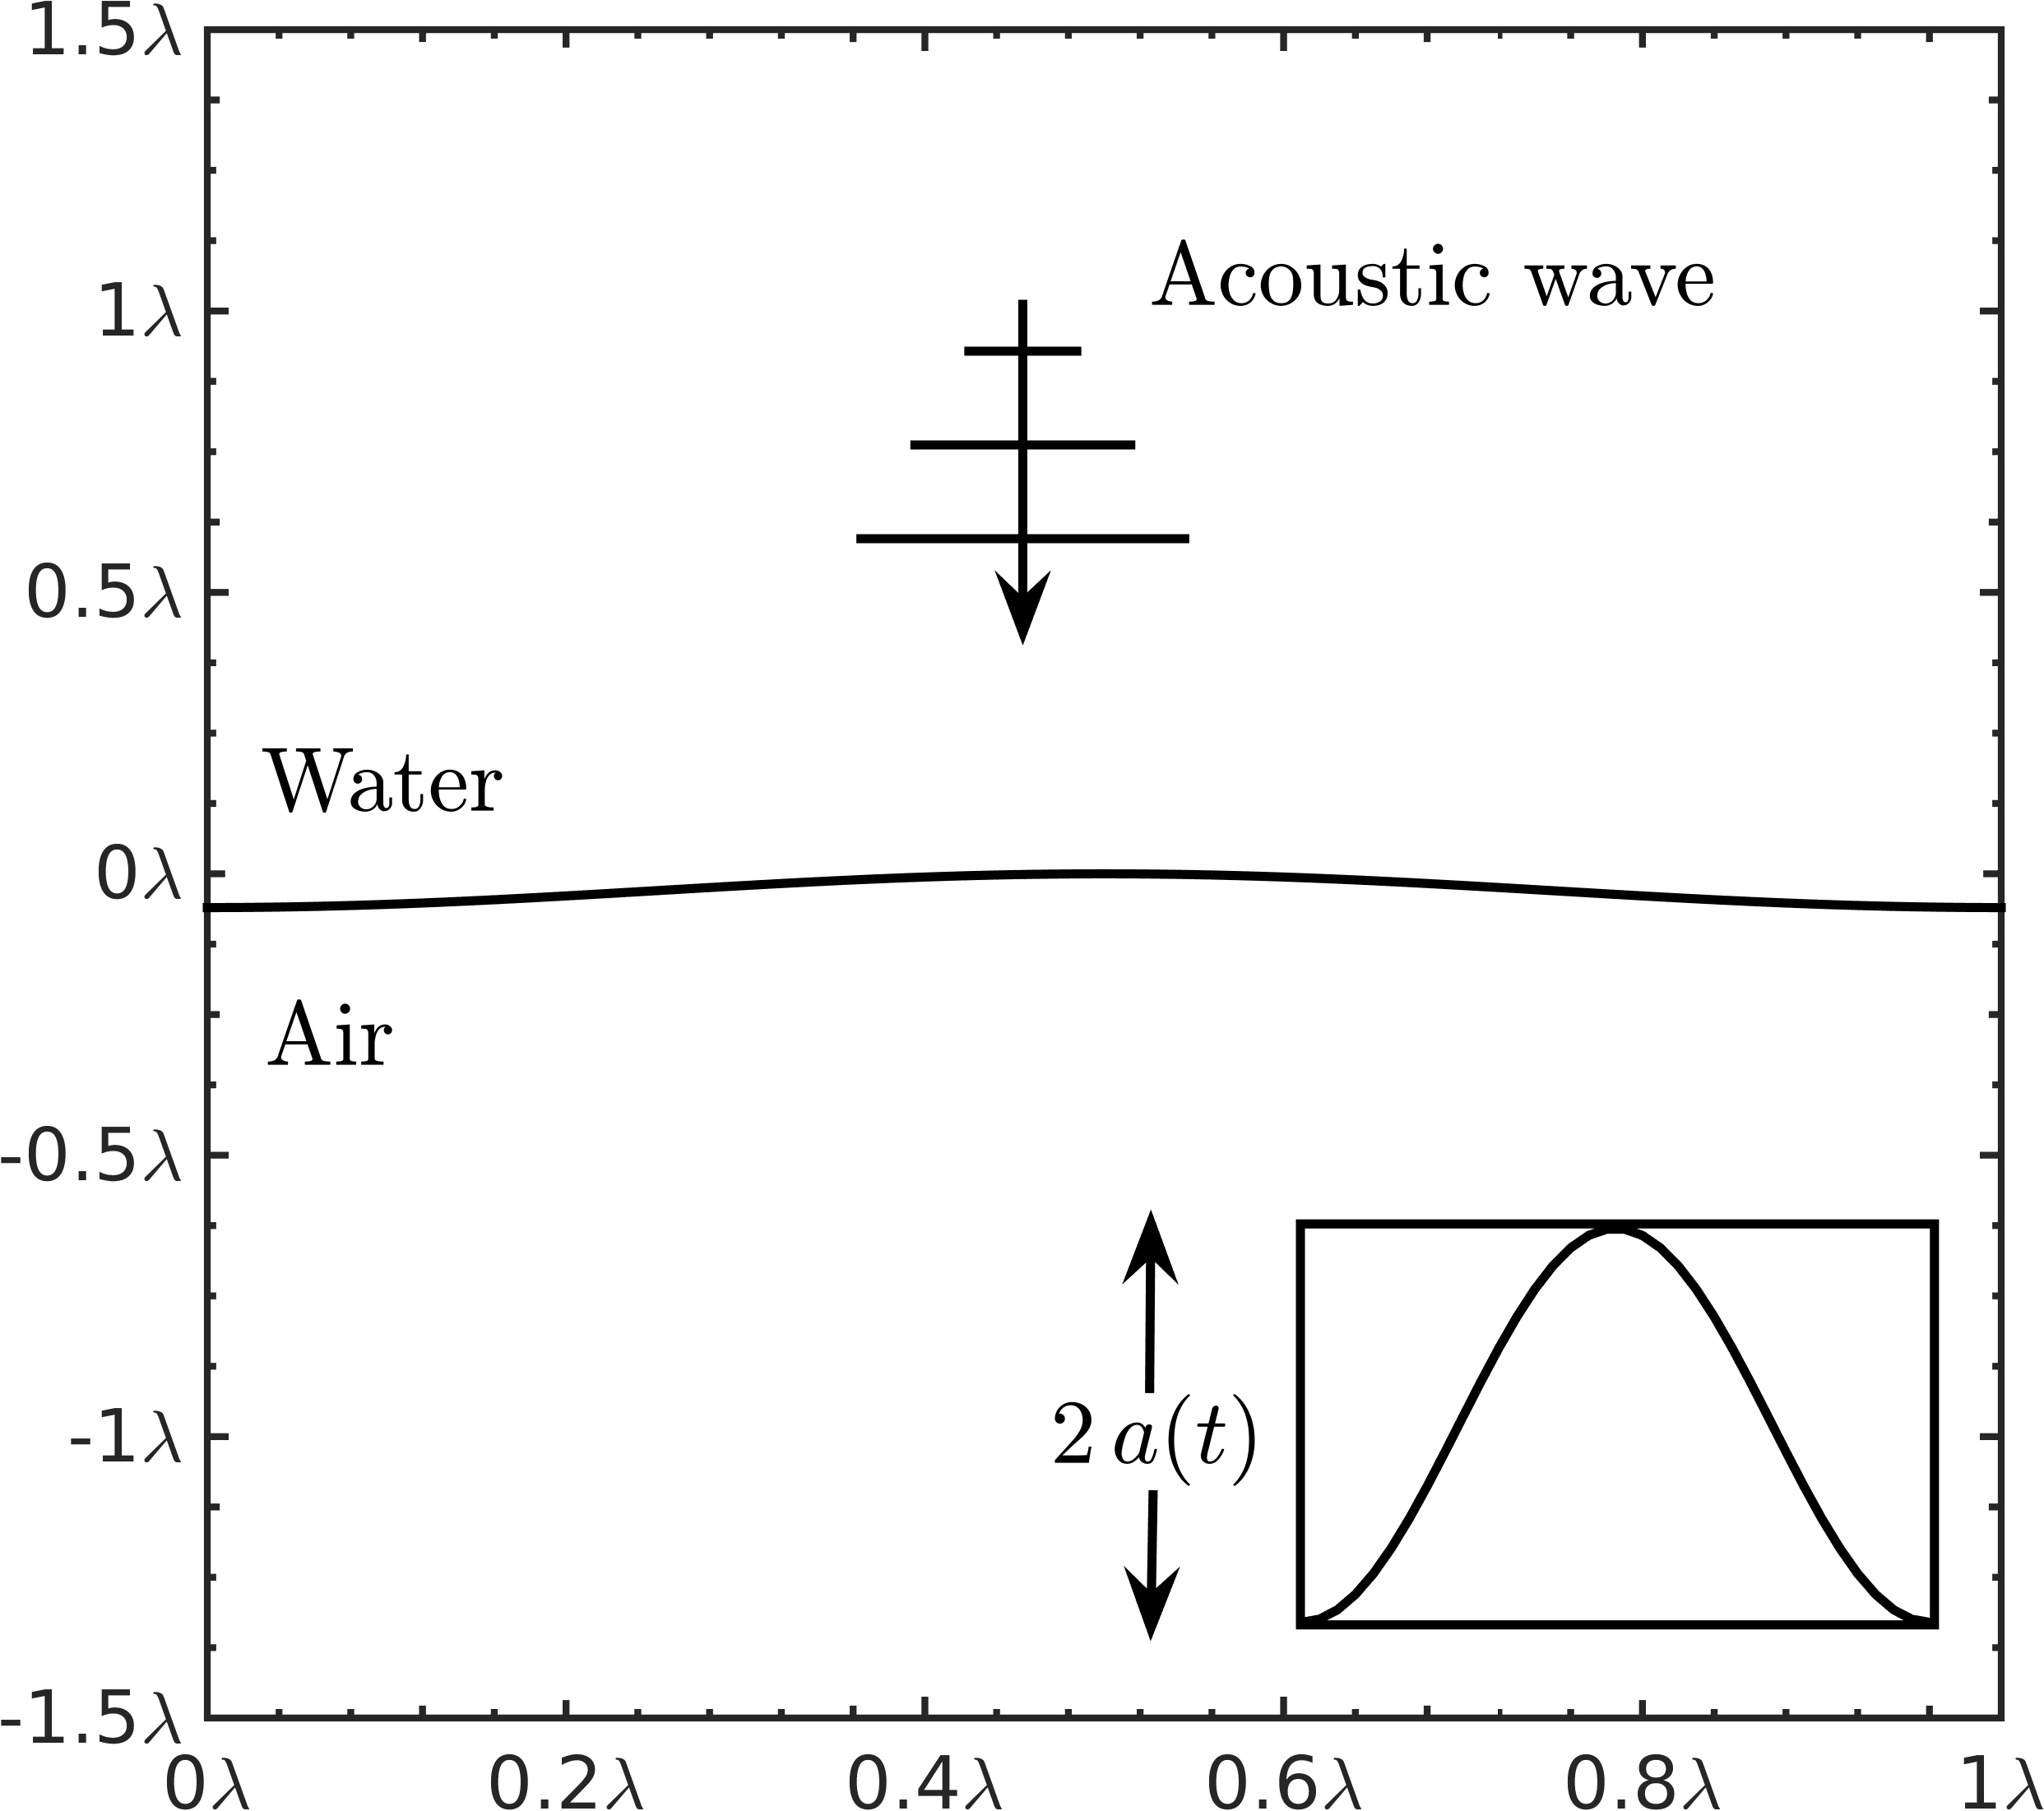
\includegraphics[width=0.4\textwidth]{./figs/lung_figs/usbe_model_schematic2} \hfill
%    \caption[A schematic view of the model problem]{A schematic of an
%      ultrasound wave impinging upon an alveolus (Left) is modeled as a
%      sinusoidally perturbed water-air interface with an acoustic wave
%      impinging from water onto the interface (Right).}
%   \label{fig:problem_schematic}
% \end{figure}
% 
Based on the described problem of interest as illustrated in Figure
\ref{fig:alveolar_schematic} and our previous considerations the
relevant physical mechanisms, we view the problem as an inviscid,
compressible fluid system. Hence we will solve the Euler Equations of
fluid motion, as described later in section
\ref{subsec:governing_equations}, and must define an appropriate
initial condition to model the problem. Thus we consider a 2D,
rectangular fluid domain in the $xy$-plane such that
$0\leq x\leq 1\ell$ and $-20\ell\leq y\leq 60\ell$. Soft tissue and
fluid surrounding the lung (modeled as water) sit atop an alveolus
(modeled as air). An acoustic wave impinges from the water downward
$(-\bs{\hat{e}}_y)$ toward the air. A schematic of the model problem
is shown in \ref{fig:problem_schematic}.

To captures the surface roughness of the alveolus, we prescribe the
initial interface to include a single-mode sinusoidal perturbation of
amplitude $a_0$ such that the vertical center of the interface is
described by
\begin{align} %Not y_interface in the code
  Y(x,t=0)_{interface} = a_0\sin\left(\frac{2\pi x}{\ell}-\frac{\pi}{2}\right),
\end{align}
hereafter referred to as $Y_{0,interface}$. For this study
$a_0=0.03\ell$ is used as a base value, though we explore the effects
of this amplitude for cases of $a_0=0.1\ell, 0.2\ell\ 0.3\ell$ where
specified. This interface geometry is consistent previous studies of
the \ac{RMI} \citep{Brouillette2002}. An interface thickness
$\delta=0.08\ell$ is prescribed such that above
$y\geq Y_{0,interface}+\delta/2$ the fluid is pure water, below
$y\leq Y_{0,interface}-\delta/2$ is pure air. In the region
$Y_{0,interface}-\delta/2 < y < Y_{0,interface}+\delta/2$, the fluid
consists of an air-water mixture, the specific treatment of which is
described later in section \ref{subsec:governing_equations}.

While our motivation is rooted in ac{DUS} of the lung, a typical
\ac{DUS} pulse is mathematically complicated and not ideal for
understanding the fundamental physics of acoustically-driven perturbed
liquid-air interfaces. Hence, we must build a simpler acoustic
waveform. To do this, we consider the differences between a \ac{DUS}
acoustic pulse and a shock, the most well studied wave for this type
of problem. We seek to create an acoustic waveform that interaction
with the interface can be partially explained studied using previously
established principles for shock-driven interfaces. We identify three
key conditions that are met by an acoustic pulse that are not met by a
shock. 1) Although sometimes highly nonlinear, \ac{DUS} pulse waves
are continuous, unlike shock waves. 2) Acoustic waves interact with
the interface over a finite time span, whereas shocks are typically
treated as accelerating the interface instantaneously. 3) Acoustic
waves contain a finite perturbation, eventually returning a
homogeneous medium approximately to its undisturbed state after
passing. Previous \ac{RMI} studies have typically considered shock
waves that leave the post-shock region in a state of elevated
pressure, velocity, etc... 

To build our waveform we start from a shock wave and adjust to meet
the three listed conditions. To uphold continuity within the wave, we
allow the acoustic pressure to increase linearly to a maximum
amplitude $p_a$ over a fixed region, $\Delta L_a$. As we are
interested in baroclinic vorticity, we choose $\Delta L_a$ such that
the acoustic pressure gradient is $\nabla p=p_a/\Delta L_a$ is roughly
consistent with that of \ac{DUS}. We assume that acoustic pressure
changes occur over a physical length on the order of the acoustic
wavelength $\lambda\approx 1$ for a $1.5$ MHz pulse. Thus for an
alveolus of diameter $200 \mu$ m, the expected pressure gradient is
$\nabla p=p_a/\lambda/2=p_a/5\ell$. Hence $\Delta L_a=5\ell$. To meet
the third condition, we eventually let the acoustically perturbed
quantities, $p, v, \rho$ fall over a length $\Delta L_a=5\ell$. To
meet the second condition we seek to have our wave interact with the
interface for a typical \ac{DUS} pulse duration, which we previously
established to have a corresponding spacial length of $45\ell$. Thus
we arrive at an initial condition for our a acoustic waveform as a
trapezoidal wave that rises in pressure from $p_{atm}$ to $p_a$ over a
length $5\ell$ remains static over a length of $35\ell$ and then drops
back to $p_{atm}$ over a final $5\ell$. This process by which we
arrived at this waveform and the final waveform itself is illustrated
in Figure \ref{fig:p0}. In choosing appropriate $p_a$ values for the
numerical experiments performed in this study, we do not limit
ourselves to strictly to acoustic parameters relevant to \ac{DUS} and
we will consider values of $p_a$ including $1, 5, 7.5, 10,$ and $15$
MPa. Unless otherwise stated, $p_a=10$ MPa for the results provided.
\begin{figure}% 
  \centering%
  \begin{subfigure}[b]{0.45\textwidth}
    \centering
    \raisebox{\height}{%
      \def\svgwidth{\textwidth}%
      \import{./figs/lung_figs/}{shock_logic_schematic.pdf_tex}%
    }%
    \caption{\label{fig:wave_logic} Design of the trapezoidal waveform}
  \end{subfigure}
  ~
  \begin{subfigure}[b]{0.5\textwidth}
    \centering
    \def\svgwidth{\textwidth}
    \import{./figs/lung_figs/}{p0_vs_y.pdf_tex}%
    \caption{\label{fig:p0_vs_y}Acoustic pressure waveform}
  \end{subfigure}
  \caption[Trapezoidal wave]{Figure \protect\subref{fig:wave_logic}
    illustrates ideological progression from a shock wave pressure
    profile to an acoustic trapezoidal wave. Three conceptual changes
    are implemented: 1) The rising pressure is spread over a finite
    distance to satisfy continuity of pressure, 2) the pressure is
    allowed to return to ambient after the passage of the wave, and 3)
    The elevated pressure is held static for a period such that the
    wave for the wave-interface interaction is of finite
    duration. Figure \protect\subref{fig:p0_vs_y} shows an example
    initial pressure condition as a function of distance from the
    interface.}%
  \label{fig:p0}
\end{figure}
% 
\subsection{Governing equations}
\label{subsec:governing_equations}
The governing equations describing the motivating problem of \ac{DUS}
of the lung are conservation of mass, momentum, and energy for a
compressible, viscoelastic material. The present work neglects elastic
and viscous effects. Thus we solve the Euler equations are presented
here for the case of fluid motion in two dimensions ($x,y$):
% 
\begin{subequations} \label{eq:euler}%
  \begin{align}% 
    \frac{\partial \rho}{\partial t} + \frac{\partial \left(\rho u\right)}{\partial x} + \frac{\partial \left(\rho v\right)}{\partial y} = 0,\\
    \frac{\partial \rho u}{\partial t} + \frac{\partial}{\partial x}\left( \rho u^2+p\right)  + \frac{\partial}{\partial y}\left( \rho uv\right) = 0,\\
    \frac{\partial \rho v}{\partial t} + \frac{\partial}{\partial x}\left( \rho uv\right)  + \frac{\partial}{\partial y}\left( \rho v^2+p\right) = 0,\\
    \frac{\partial E}{\partial t} + \frac{\partial}{\partial x}\left[u\left(E+p\right)\right] + \frac{\partial}{\partial y}\left[v\left(E+p\right)\right] = 0,
  \end{align}%
\end{subequations}%
% 
where $t$ is time, $\rho$ is density, $p$ is the pressure, $u$ and $v$
are the velocity components in the $x$ and $y$ directions
respectively, and $E$ is the total energy. To close the system, we
use a stiffened equation of state to relate the total energy to the
pressure and velocity in the flow, such that,
% 
\begin{align} \label{eq:stiffened_eos}%
  E=\frac{\rho\left(u^2+v^2\right)}{2} + \frac{p+n B}{n-1}.
\end{align}
% 
Here $B$ is a measure of liquid stiffness that has been experimentally
determined for this equation. For perfect gases, such as is our
treatment of air, $n$ is the specific heats ratio and $B=0$. The
sound speed in our simulations is calculated based on the following
relationship, derived from the stiffened equation of state.
% 
\begin{align} \label{eq:sound_speed}%
  c = \sqrt{\frac{n\left(p+B\right)}{\rho}}.
\end{align}
% 
While physical diffusion is not considered in this setup, portions of
the flow contain a water-air mixture as a result of the initial
treatment of the interface and numerical diffusion. The numerical
treatment of the diffusion layer at the interface for the initial
condition is such that the density has an exponential profile
\citep{Latini2007}, which is used to get the mass fraction and
molecular weight fields in the mixed region. These are then used to
determine the initial conditions for $n$ and $B$ in a
thermodynamically consistent fashion.

To solve for the material parameters in the mixed region and prevent
spurious pressure oscillations at the interface, two additional
advection equations are solved for $n$ and $B$.
\begin{subequations} \label{usbe_lung_eosvar_advection}%
  \begin{align}% 
    \frac{\partial}{\partial t}\left(\frac{n B}{n-1}\right)+u\frac{\partial}{\partial x}\left(\frac{n B}{n-1}\right)+v\frac{\partial}{\partial }\left(\frac{n B}{n-1}\right) = 0,\\
    \frac{\partial}{\partial t}\left(\frac{1}{n-1}\right)+u\frac{\partial}{\partial x}\left(\frac{1}{n-1}\right)+v\frac{\partial}{\partial y}\left(\frac{1}{n-1}\right) = 0. 
  \end{align}%
\end{subequations}%
This implementation is consistent with the works of \cite{Abgrall1996,
  Shyue2001, Beig2015}. Details of the full numerical implementation
are explained by \cite{HenrydeFrahan2015}.
%
\subsection{Computational  methods}%
\label{subsec:numerical_methods}%
Before solving the system of governing equations presented we
non-dimensionalize by the density and sound speed of air (provided
below). It is worth noting that the Euler equations are length scale
invariant, and thus no inherent physical length scale exists in the
equations that we solve. Hence reason that all length scales are
defined in terms of the to the alveolar length scale $\ell$, which is
also the initial interface perturbation wavelength and the width of
the computational domain.

The dimensional fluid properties used for air determined at a
temperature of $300$ K and an $1$ atm of pressure such that
$\rho^*_{air}=1.18$ (kg/m$^3$). The stiffened equation of state
variables are given by $n_{air}=1.4$ and $B^*_{air} = 0$ (Pa) such
that $c^*_{air}=347.2$ (m/s) based on equation
\eqref{eq:sound_speed}. For water, $\rho^*_{water}=996$ (kg/m$^3$) and
the stiffened equation of state variables have been determined
empirically and are given by $n_{water}=5.5$ and
$B^*_{water} = 492115000$ (Pa) such that $c^*_{water}=1648.7$ (m/s)
\citep{Marsh1980,holian1984t,Cocchi1996}. Non-dimensionalizing these
values based on the density and sound speed of air presented we find
that $\rho_{air}=1$, $B_{air} = 0$, $c_{air}=1$, and
$\rho_{water}=846.6$, $B_{water} = 3469.1$, and $c_{water}=4.75$.
 
To solve the governing equations, we implement a third-order accurate
\ac{DG} scheme in space and a fourth-order accurate, adaptive
Runge-Kutta method to march forward in time
\citep{HenrydeFrahan2015}. Roe solver is used to calculate flux in and
out of each cell in a way that handles discontinuities and keeps the
interface sharp. The grid resolution is 100 points per $\ell$ unless
otherwise stated. To minimize artificial reflections, we use inflow
and outflow boundary conditions at the top and bottom of the domain,
and implement geometric grid stretching in the vertical direction for
the top and bottom-most $10\ell$ segments of the grid. Periodic
boundary conditions are used at the left and right edges of the
domain.

%%% Local Variables:
%%% mode: latex
%%% TeX-master: "../main"
%%% End: